\documentclass{beamer}
\usepackage[ngerman]{babel}
\usepackage[utf8]{inputenc}
\usepackage{natbib}
\usefonttheme{professionalfonts}
\usetheme{Boadilla}

\begin{document}
\title[Adaptive Gestenerkennung]{Adaptive Gestenerkennung mit Variationsabschätzung für interaktive Systeme}
\author{Maxim Boianetchii \and Marian Stein}
\date{\today}
%\institute{Universität Rostock}

\begin{frame}
\titlepage
\end{frame}

\begin{frame}\frametitle{Motivation}
\begin{itemize}
\item Gestenerkennung in vielen Gebieten gefragt:
\begin{itemize}
\item Medizin
\item Automobilindustrie
\item Unterhaltungsbranche
\end{itemize}
\item Mit aktuellen Methoden nur eingeschränkt möglich
\begin{itemize}
\item Erkennung teilw. nur nach vollst. Ausführung der Geste
\item Keine Rückmeldung von Zusatzinformationen über die Geste(z.B Geschwindigkeit)



\end{itemize}
\end{itemize}
\begin{columns}
\begin{column}{0.4\textwidth}
\begin{figure}
\centering
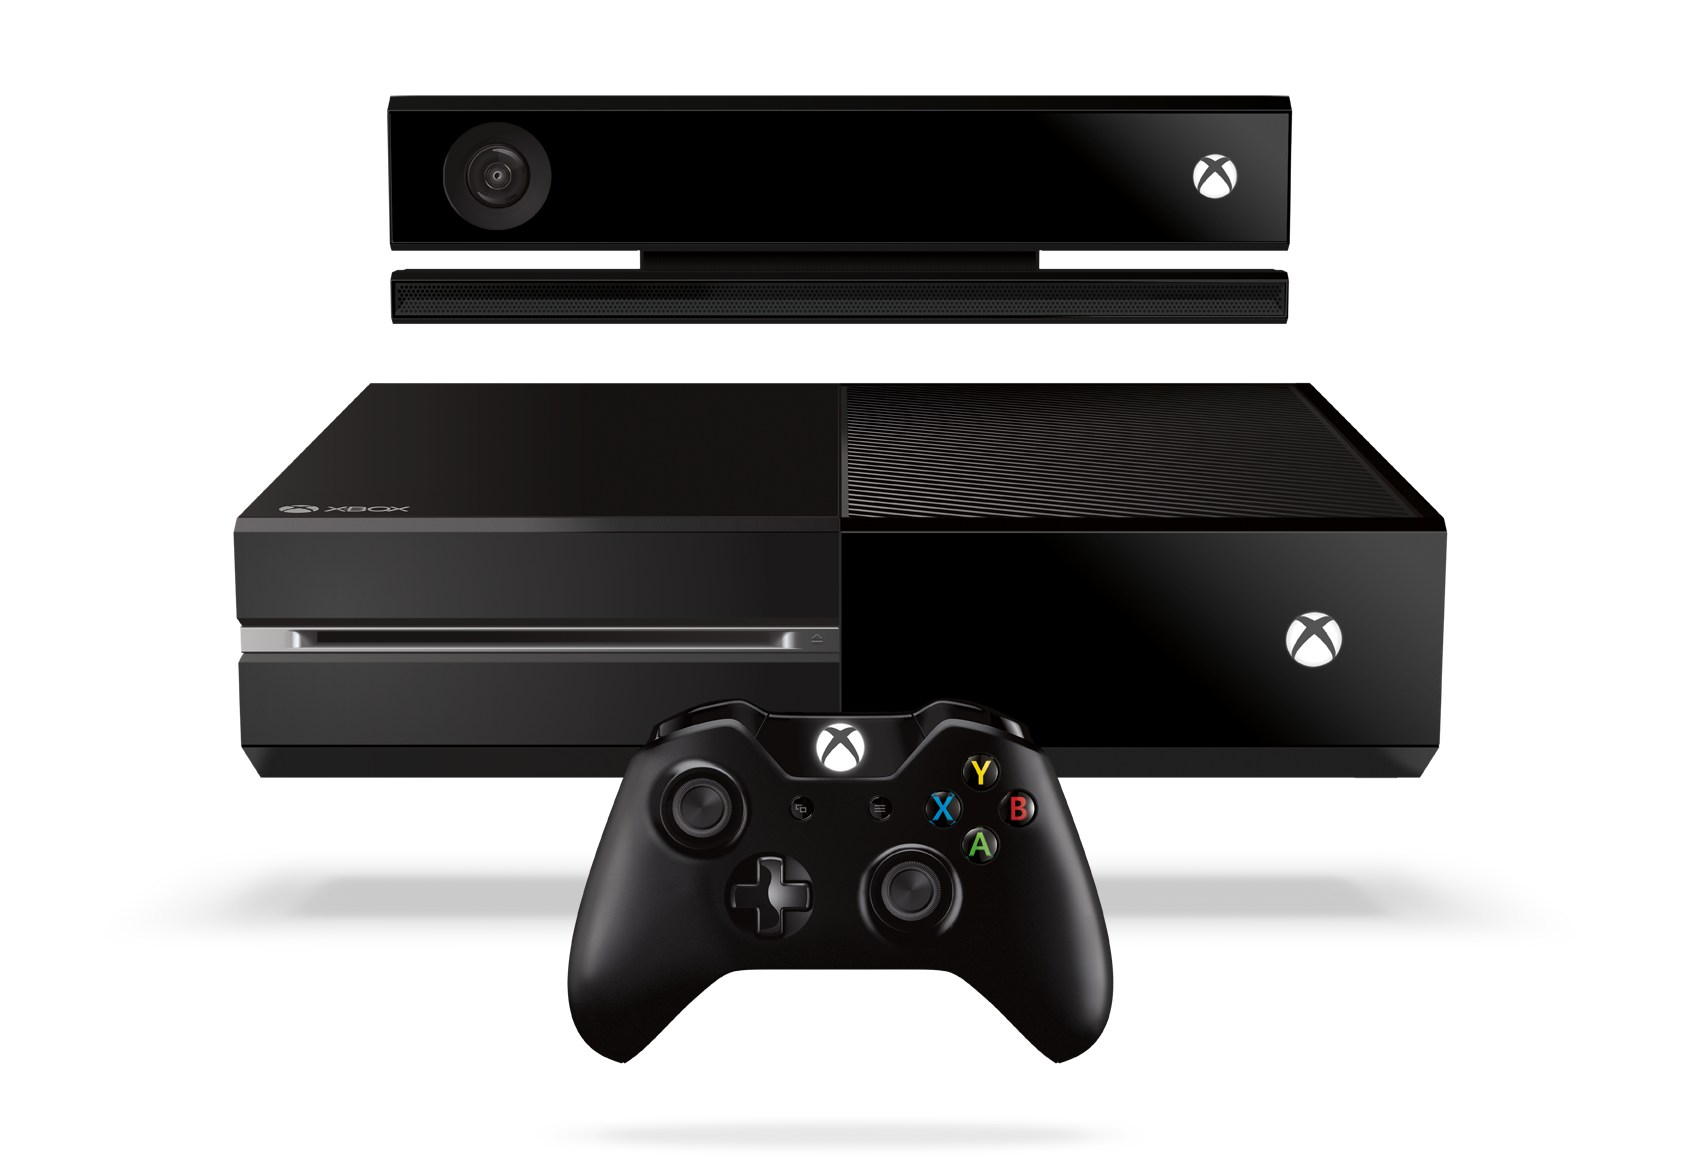
\includegraphics[width=0.7\linewidth]{../Bilder/xbox}
\label{fig:xbox}
\end{figure}
\end{column}
\begin{column}{0.4\textwidth}
\begin{figure}
\centering
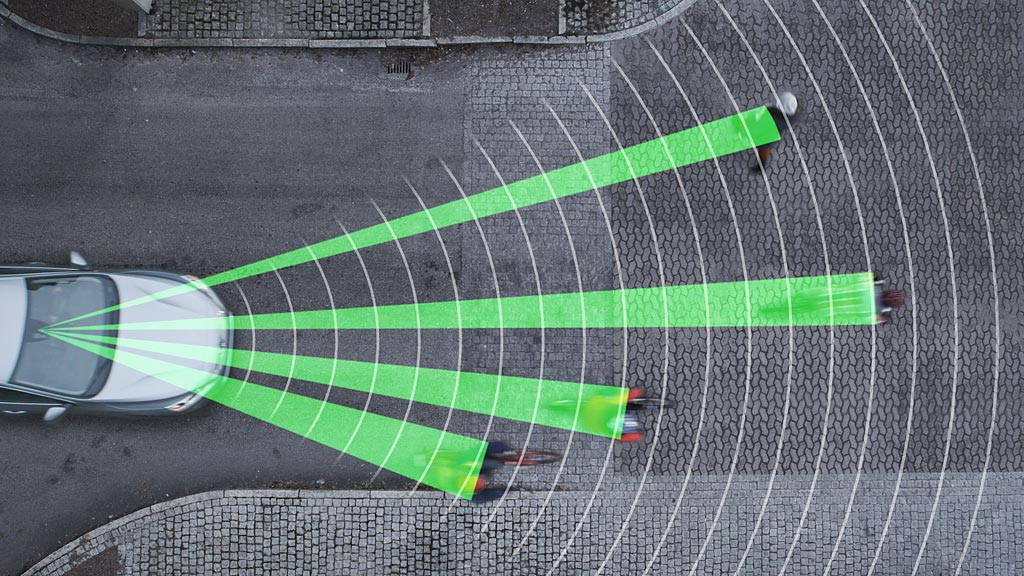
\includegraphics[width=0.7\linewidth]{../Bilder/fussgaenger}
\label{fig:fussgaenger}
\end{figure}
\end{column}
\end{columns}
\end{frame}
\begin{frame}\frametitle{Vorgeschlagene Methode}
\begin{itemize}
\item Verwendung eines Partikelfilters
\item frühzeitige Erkennung und Rückmeldung von Variationsinformationen, z. B. Geschwindigkeit, Drehung, etc.
\begin{itemize}
\item Ermöglicht Anwendungen, bei denen die Benutzer direkt während der Gestenausführung interagieren können
%Verweis auf Nutzerstudie
\end{itemize}
\end{itemize}
\end{frame}
\begin{frame}\frametitle{Ähnliche Arbeiten}
\begin{itemize}
\item Templatebasierte Erkennung (\citet{Wobbrock2007}):
\begin{itemize}
\item Vorverarbeitung der aufgenommenen Daten
\item Erkennung mithilfe euklidischen Abstands
\end{itemize}
\item Dynamic Time Warping(\citet{Gawrila1995,Liu2009})
\begin{itemize}
\item Erfassung der gesamten Geste
\item Anpassung durch Strecken/Stauchen der Vorlage
\end{itemize}
\item Kondensationsalgorithmus (\citet{BlackandJepson1998a})
\begin{itemize}
\item gleiche Grundidee wie der vorgeschlagene Algorithmus
\item Anpassung auf Skalierung beschränkt
\end{itemize}
\end{itemize}
\end{frame}

\begin{frame}\frametitle{Interaktionsprinzipien}
\begin{columns}

\begin{column}{.55\textwidth}
\begin{itemize}
\item neue Interaktionsmöglichkeiten:
\begin{itemize}
\item Tonmanipulation
\item Viedospiele
\item etc.
\end{itemize}
\item zwei grundlegende Interaktionen:
\begin{itemize}
\item Ausführung/Festlegung der Geste
\item Manipulation der Geste während der Ausführung
\end{itemize}
\item Erkennung der Geste und Abschätzung der Variationen in Echtzeit und kontinuierliche Aktualisierung
\item Verwendung eines einzigen Templates pro Geste
\end{itemize}
\end{column}
\begin{column}{.4\textwidth}
\begin{figure}
\centering
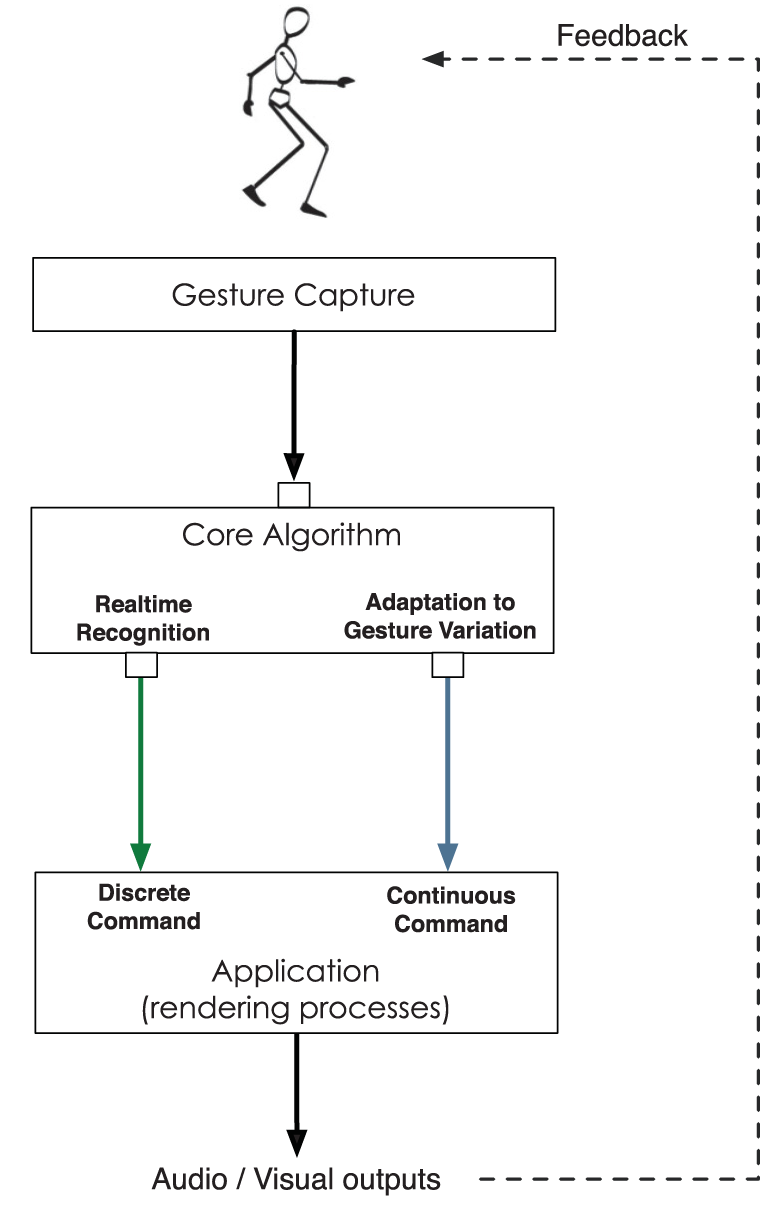
\includegraphics[width=\linewidth]{../Bilder/Fig1}
\label{fig:Fig1}
\end{figure}
\end{column}
\end{columns}
\end{frame}

\begin{frame}\frametitle{zugrundeliegendes Modell}
\begin{itemize}
\item Geste: Gliedmaßenbewegung, die durch eine Zeitserie einer festen Anzahl parameter Vertreten wird
\item Zustandsmodell zum Zeitpunkt $k$:
\begin{equation}
\left\{\begin{array}{l}
x_k = f_{TR} (x_{k-1}, v_{k-1}) \\
z_k = f_{OB} (x_k, w_k; g) \\
\end{array}\right.
\end{equation} 	
\begin{itemize}
\item $x_k$: Vektor des Systemzustands, mit den Gestenparametern als Elemente
\item $f_{TR}$ Funktion für die Entwicklung des Zustands, abhängig vom vorherigen Zustand und der Abweichungssequenz $v_k$
\item $f_{OB}$ Funktion, die aus den Messwerten $w_k$, dem vorherigen Zustand und einer Tempplategeste $g$ Beobachtungen generiert
\end{itemize}
\end{itemize}
\end{frame}

\begin{frame}\frametitle{zugrundeliegendes Modell}
\begin{columns}
\begin{column}{0.4\textwidth}
\begin{itemize}
\item Die ersten 2 Elemente des Zustandsvektors $x_k$ werden festgelegt als Phase und Geschwindigkeit, weitere Elemente können weitere Parameter enthalten
\item $f_{TR}$ ist linear und gaussverteilt
\item $f_{OB}$ wird durch eine Student'sche t-Verteilung modelliert
\end{itemize}
\end{column}
\begin{column}{0.6\textwidth}
\begin{figure}
\centering
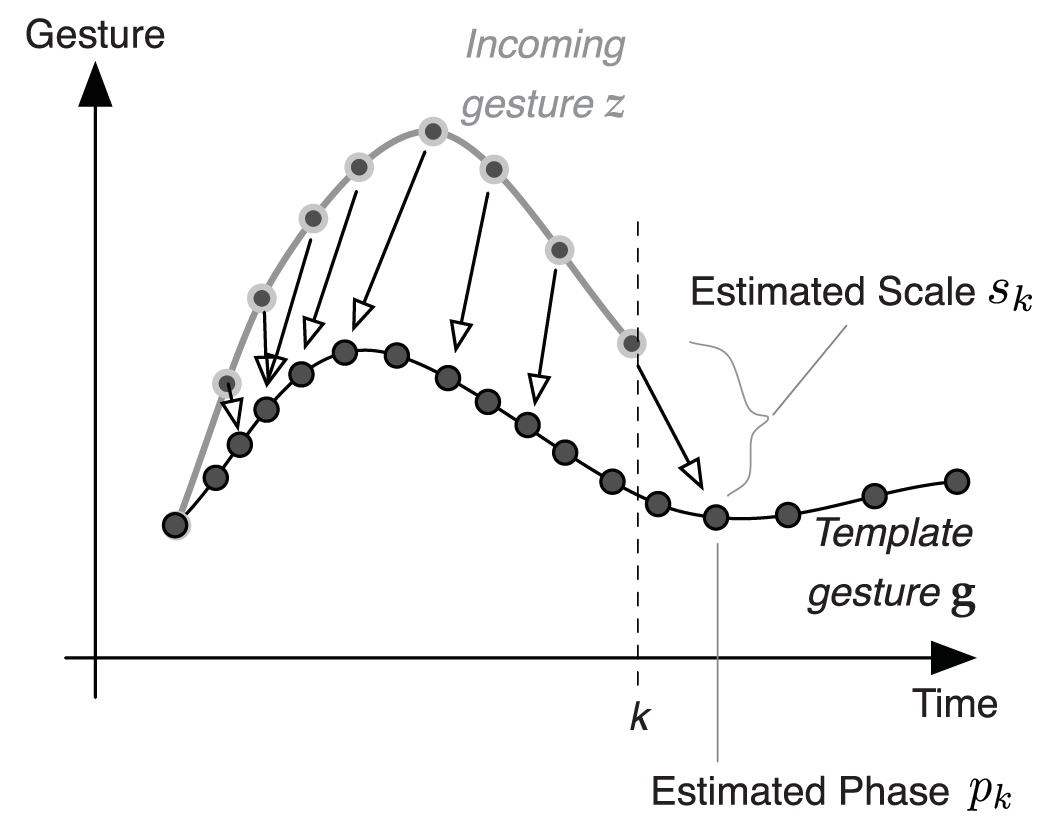
\includegraphics[width=\linewidth]{../Bilder/Fig2}
\label{fig:Fig2}
\end{figure}
\end{column}
\end{columns}
\end{frame}

\begin{frame}\frametitle{zugrundeliegendes Modell}
\begin{itemize}
\item Inferenz des Zustandsvektors mithilfe eines Partikelfilters
\begin{itemize}
\item Zustand wird durch Gewichtung vieler, in diesem Fall gaussverteilter, Partikel abgeschätzt
\item jedes Partikel repräsentiert einen möglichen Zustand und wird mit seiner Wahrscheinlichkeit gewichtet
\item Gewichtung der Partikel wird durch $f_{OB}$ beeinflusst
\end{itemize}
\item Der erwartete Gesamtzustand ist dann durch die gewichtete Summe aller Partikel gegeben
\item Um zwischen verschiedenen Gesten zu unterscheiden, wird der Zustandsraum um einen Gestenindex erweitert und die Partikel gleichmäßig über alle Gestenindizes verteilt.
\end{itemize}
\end{frame}

\begin{frame}\frametitle{Literatur}
\bibliographystyle{plainnat}
\bibliography{praesentation}

\end{frame}

\end{document}